\chapter{基于图模型的方面级情感分析算法}
第三章探讨了基于图模型理论的整体文本分类算法,图模型应用于文本分类任务取得了一定效果。尤其是考虑作为全局信息而引入的超节点
对模型性能有一定的正面影响。超节点实际上不仅仅可以作为全局信息而使用,根据不同任务可以设置不同类型的超节点。本章依旧基于图模型
理论,探讨关于方面级情感分析的任务。本章算法超节点不再使用全局信息而使用方面词信息,并与第三章构图方式一致,建立文本图结构,实现方面级
情感分析。

\section{引言}
方面级情感分类\citing{zhou2019deep}已经越来越备受关注,相比于一般的文本分类算法具有更高的实用性。例如对于在美团、京东、天猫等平台上进行的商品评价描述,
采用方面级的情感分类可以针对商品不同的方面进行评价,进而实现对产品全方位的点评,并且平台可以根据点评的方面以于分类,以保障用户对不同方面的感知和需求。
比如有些用户看重服务,有些用户看重质量。同时商家可以根据用户对不同方面的评价进行改进,提升商品整体质量。方面级情感分类相比于一般的文本分类算法,具有一定难度。

Li等人\citing{li2018transformation}使用一个Bi-LSTM模型处理文本序列,获取每个单词的中间隐藏状态的向量表示,随后每个单词向量对应一个CPT结构(Context-Preserving Transformation)。
每个CPT中采用Bi-LSTM模型学习一个方面词对应的信息向量然后与输入的单词向量拼接获取一个新的单词向量,该向量体现了每个单词与目标词之间的关系信息。
通过CPT层后,每个单词具有一个新的向量表示,再对这组向量表示采用CNN模型卷积处理,捕捉关键信息,生成表示文本的向量,用以实现分类。
Wang等人\citing{wang2016attention}提出了一个基于LSTM的注意力机制模型。它将方面词的向量表示分别与文本内容的每个单词向量表示进行拼接,组合成新的向量,作为LSTM模型的输入。
随后将LSTM模型获得的每步单词的隐藏状态与方面词向量用一个注意力机制求得权重,代表了每个单词对目标情感的贡献度。最后通过向量加权和表示最终的用以分类的向量表示。虽然
这些方法取得了一定效果,但是使用不能并行计算的LSTM模型,计算效率相对较低。同时方面级的目标词与文本内容单词之间应该存在许多联系,
如果能够挖掘它们之间的内在关系,便能进一步学到情感信息。

本章基于第三章提出的图模型算法,进一步改进使之适合方面级情感分析任务。具体来说,本章的算法不再使用依据语料库信息构建超节点,而是使用对应的方面词构建,即希望这个超节点学习到的
是方面词信息,同时将这个信息通过图结构传递给其他单词节点。文本图其他部分构建过程采用第三章描述的方式一致。考虑到门控机制具有选择遗忘的功能,而图卷积神经网络
每一层的节点信息对于下一层并不一定都有用,因此,本章采用一个门控机制去控制每层节点信息的流动。通过图模型学习,将获得每个单词新的向量表示以及一个表示为方面词的信息向量。
方面词的具体情感信息取决于文本中对应位置的情感词汇,因此,本章继续采用一个注意力机制,通过方面词向量去查询所有单词中对它情感偏向最重要的词汇,获得相应的权重,最后将这些向量进行
加权和,得到最终的用以实现分类任务的向量。

综上所示,本章提出的方法主要有以下三点特色:\noindent\textcircled{1}采用一个超节点表示方面词信息,并将这个信息通过图网络进行传递,进而捕捉文本单词以及方面词之间的关系,学到两者的向量表示。
\noindent\textcircled{2}通过门控机制选择或遗忘传递给图模型中下一层的信息。\noindent\textcircled{3}利用注意力机制寻找对目标词情感贡献最大的词汇。

\section{问题定义}
本章主要探讨的是方面级情感分类任务。对于这类任务不同于整体文本分类任务,每个文本中都有一个或多个方面词。如句子“great food but the service was dreadful”,这个句子中定义
了两个方面词一个是“food”,另一个是“service”,方面级情感分类任务的目标就是判断这两个方面词对应的情感倾向。如“food”这个词,采用“great”进行形容,是一个褒义词,因此对于“food”的情感
可以归属于正向的。而对于“service”这个词,是使用“dreadful”进行描述的,属于贬义词,因此情感归属于负面。

某一文本数据$T_i$由一组$n$个单词以及多个方面词构成,$T_i=[w_1,a_{i}...a_{j},w_{n-1},w_n]$。其中$w$表示一个单词,$a_i$表示为第$i$个方面词,通常方面词由一个或多个单词组成。
文本中每个单词都有一个对应的单词向量,本章采用的单词向量主要是从Glove或经过BERT模型后得到。因此一个文本可以由一个$\mathbb{R}^{n\times d}$的向量矩阵表示,其中$n$
表示文本中单词的个数,$d$表示为单词向量的维度。方面级情感分类任务就是学得一个函数$F(\cdot)$,输入这段文本以及需要分析的这段文本中的方面词,输出这个方面词对应的情感倾向,即判断
这个方面词是正向的或是负面的或是无情感。

\section{算法模型设计}
以前的一些研究仅仅直接对方面词的向量以及文本向量进行拼接,并未细致考虑方面词与文本中其他单词之间的联系。如果能够挖掘它们之间的内在关系,便能进一步提升模型性能。此外在图卷积网络计算中
,网络层数的增加意味着当前节点将会获取得到更远处节点的信息。而更远处节点的信息不一定对当前节点有用,因此本章采用一个门控机制,选择性的选择或是遗忘节点信息,控制信息流动,进一步提升模型
性能,确保学到更有效的向量表示。注意力机制使得模型关注于重要信息,查找对于方面词情感分析更为重要的词汇。本节主要详细阐述了算法模型,命名为GAGCN,首先介绍了模型的整体设计,之后再详细介绍
每一步的具体实现。

\subsection{模型总览}
本章实现的方面级情感分析算法流程图如图\ref{asgraphLct}所示。预处理是指对文本数据进行统一的规则化处理,首先将所有文本都处理成小写字体,同时删除部分无关的词汇,比如一些停止词等。
建立词汇表,不同的单词应该对应一个唯一的索引,有助于后期处理时正确找到每个单词所对应的嵌入向量。同时需要标注每个文本中对应的方面词所在位置,便于后续分析任务使用。
\begin{figure}[htb]
	\setlength{\belowcaptionskip}{0pt}
	\centering
	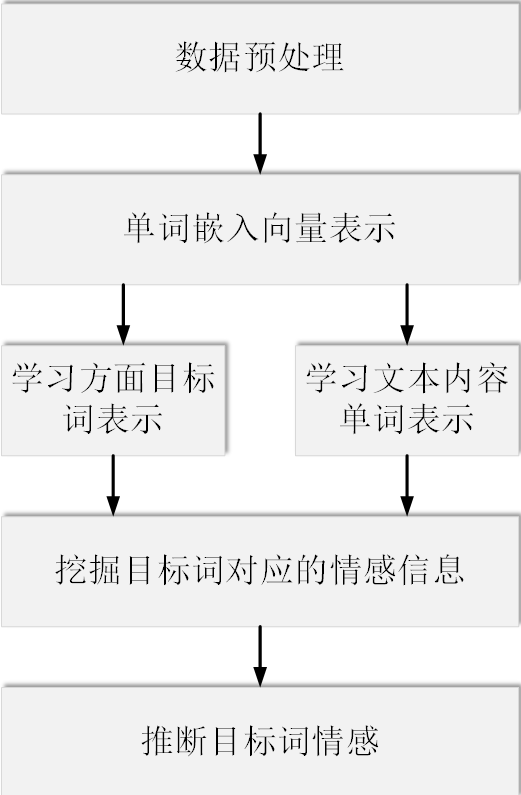
\includegraphics[width=0.3\textwidth]{pic/asgraph.png}
	\caption{方面级情感分析算法流程图}
	\label{asgraphLct}
\end{figure}
方面词向量以及文本单词向量的学习都是基于图网络模型,经过图卷积神经网络学得到一个超节点向量,即表示为方面词向量,以及每个单词的新的向量表示。方面词关键词汇信息挖掘即是使用注意力机制
关注重点词汇,找出对该方面词的情感倾向有帮助的词汇,最后实现分析。

本章提出的方法是一个端到端的深度学习模型,即输入文本内容和对应的方面词,就可得到该方面词对应的情感类别。该算法总共有三个部分,如图\ref{asgraphart}所示,第一部分定义为文本构图部分,
该步骤主要是将文本中的单词采用第三章提到的构图方法构建成图,其次构造一个传递方面词信息的超节点。第二部分主要是单词词向量表示学习以及超节点的表示学习,这部分采用基于多头注意力机制的GCN
进行学习以及一个门控机制用以控制图网络模型中每一层信息的传递。第三部分是基于第二部分学到的文本词向量以及超节点向量来计算。将超节点向量作为注意力机制中的Query向量,
计算文本单词中所有单词的权重,权重的大小即可视作这个单词对方面词情感的分析的重要程度。随后将注意力机制获得向量与超节点向量进行一个简单地结合,即得到最终的分类向量,将这个向量输入一个简单的
神经网络通过softmax激活函数实现情感分析任务。以下几节将对这些部分进行详细介绍。
\begin{figure}[htb]
	\setlength{\belowcaptionskip}{0pt}
	\centering
	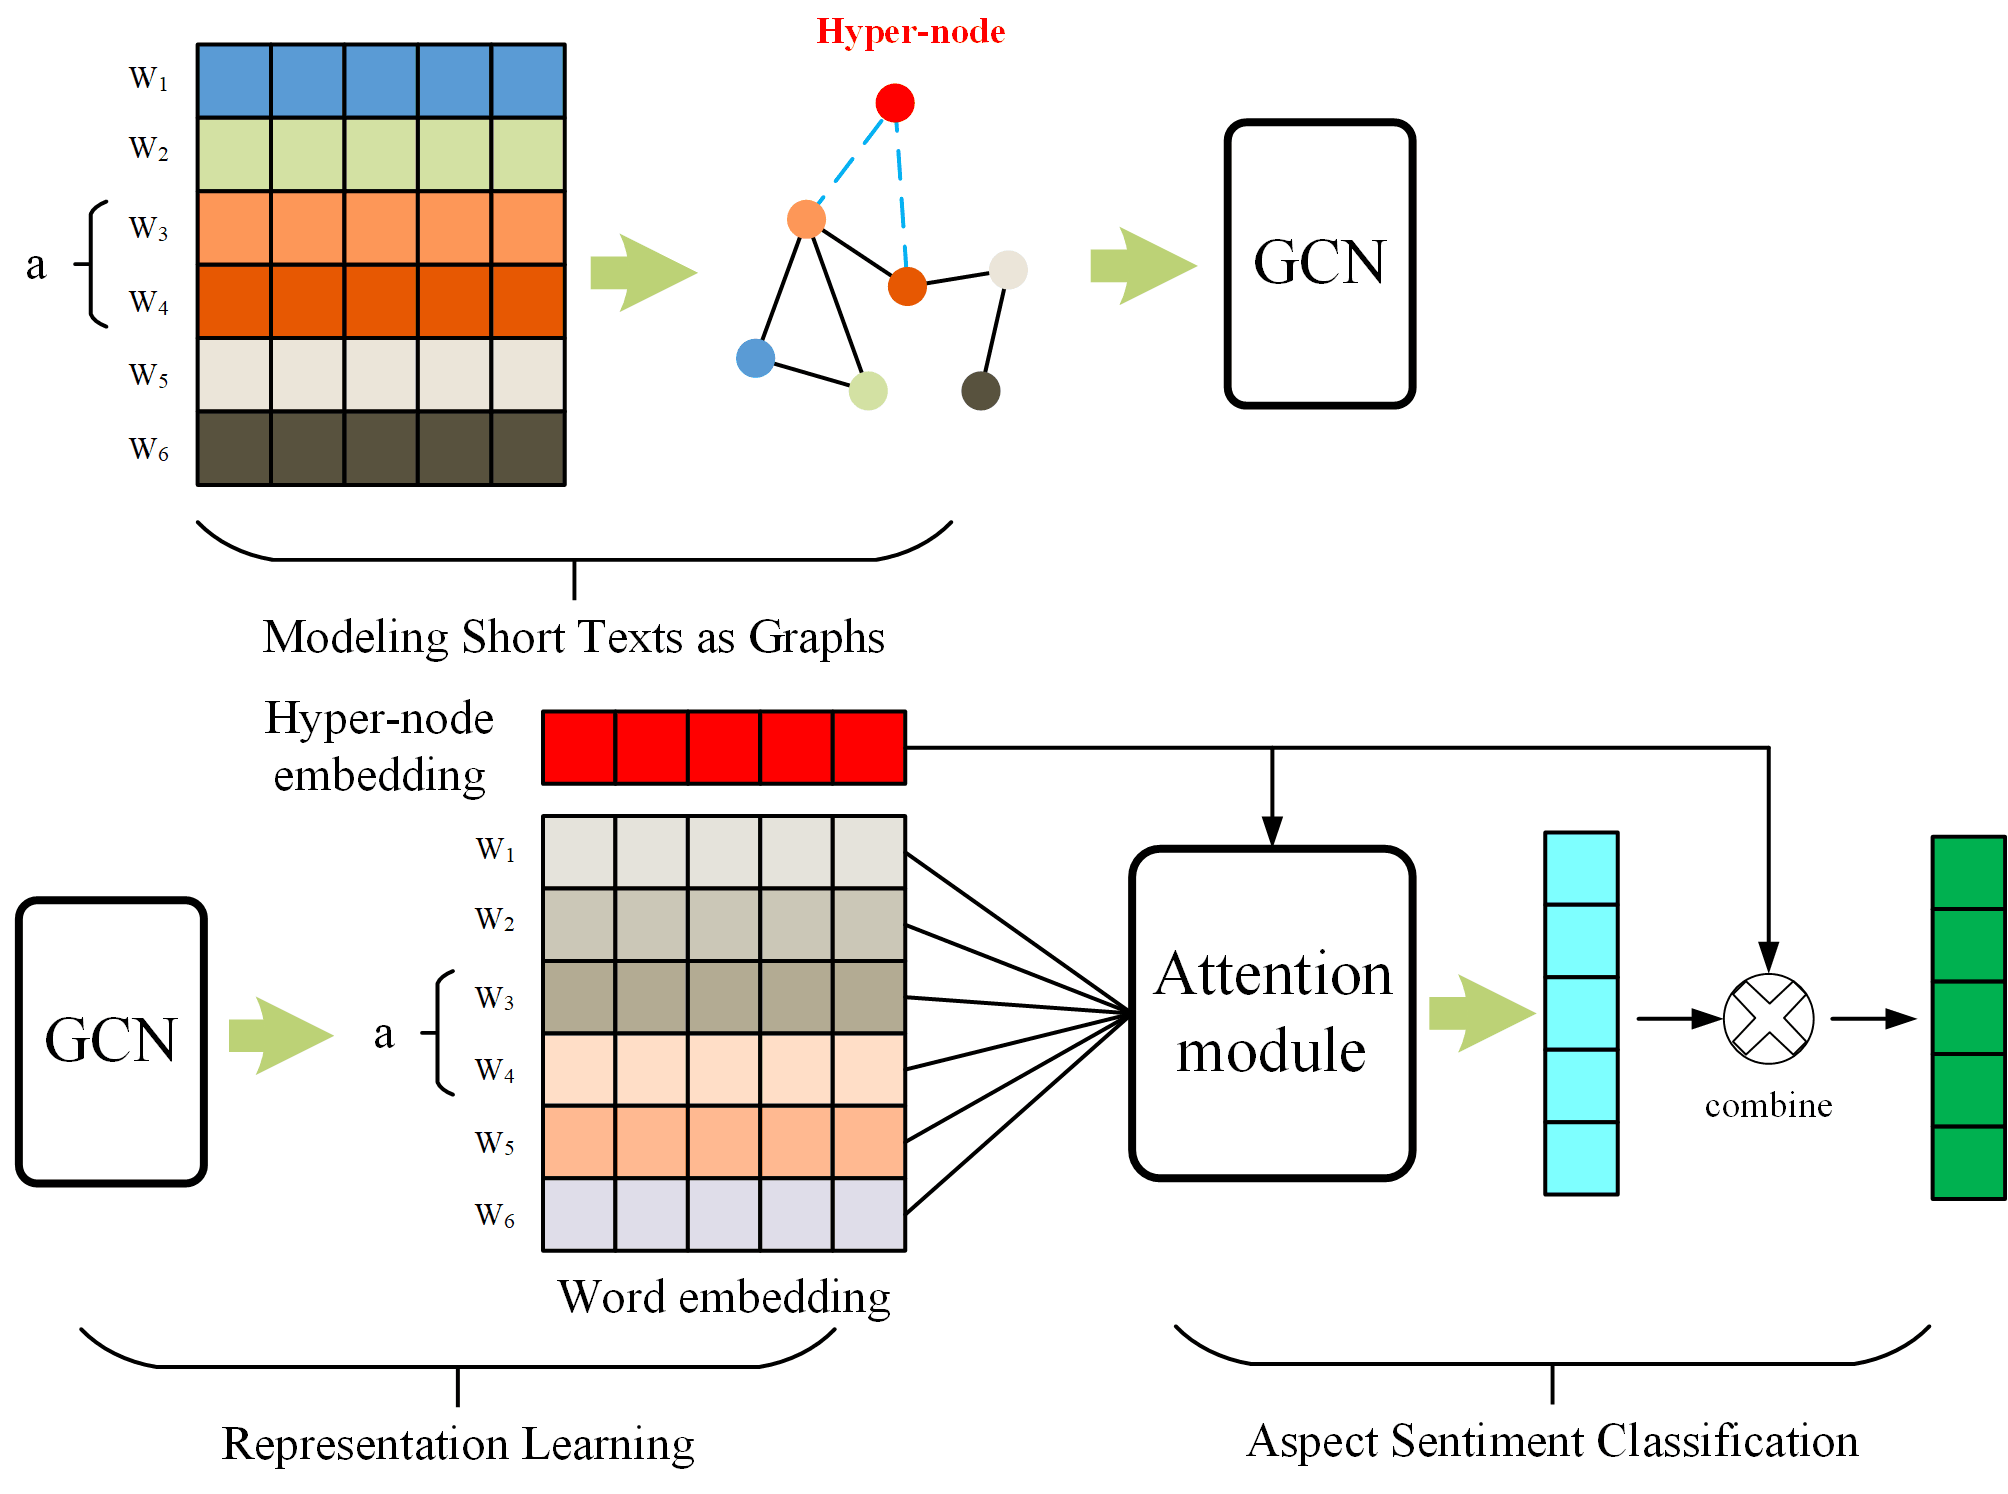
\includegraphics[width=1\textwidth]{pic/asgraphart.png}
	\caption{方面级情感分析算法模型}
	\label{asgraphart}
\end{figure}

\subsection{文本图建模过程}
本章文本图的构建过程与第三章图构建过程一致,均是采用滑动窗口的方式构建单词与单词之间的图。但与第三章略有不同,第三章中每个单词在图中仅有一个节点,即使一个单词在同一个文本中只出现了一次,
也仅仅视作一个节点。而本章中因为同时还要采用BERT预训练模型,因此构图过程中,为文本中每一个单词都构建一个节点,即使是同一个单词只要出现的位置不同,均构建一个不同的节点。单词与单词之间的边如
第三章公式\ref{weightGraph}所示。超节点不再使用TF-IDF的方式计算,构建的超节点依然是一个双向边,一向由方面词节点连向超节点,一向由超节点连接方面词。如图\ref{asgraphart}所示,图中$w_3$$w_4$是
属于方面词$a$的两个单词,超节点分别构建一条连接这两个单词节点的边,如图中虚线所示。构建时边的权重为固定值1,在图卷积计算过程中会由注意力机制更新权重,着重关注于方面词中重要的词汇。
超节点中双向边的构建有助于超节点向量传递给方面词中的每个单词,超节点向量可以视作整个方面词的信息,通过把完整的信息传递给其中的每个单词节点,有助于方面词中单词信息理解的完整度。其次,在多层的图卷积
过程中,超节点信息也能进一步传递给其他单词节点,使得其他节点也能获得方面词向量信息。这样有助于整个文本向量理解任务目标,明确需要分类的具体方面词,进而有目的性的去学习有用的词向量。


\subsection{词向量与超节点向量表示学习}
表示学习过程依然采用图卷积神经网络进行。相比于第三章提出的方法,在注意力机制计算过程进行了改进,同时还提出一个门控机制对每层传递的信息进行控制。如图\ref{attgcn}所示,假设在
每一层GCN网络中,当前需要计算的
\begin{figure}[htb]
	\setlength{\belowcaptionskip}{0pt}
	\centering
	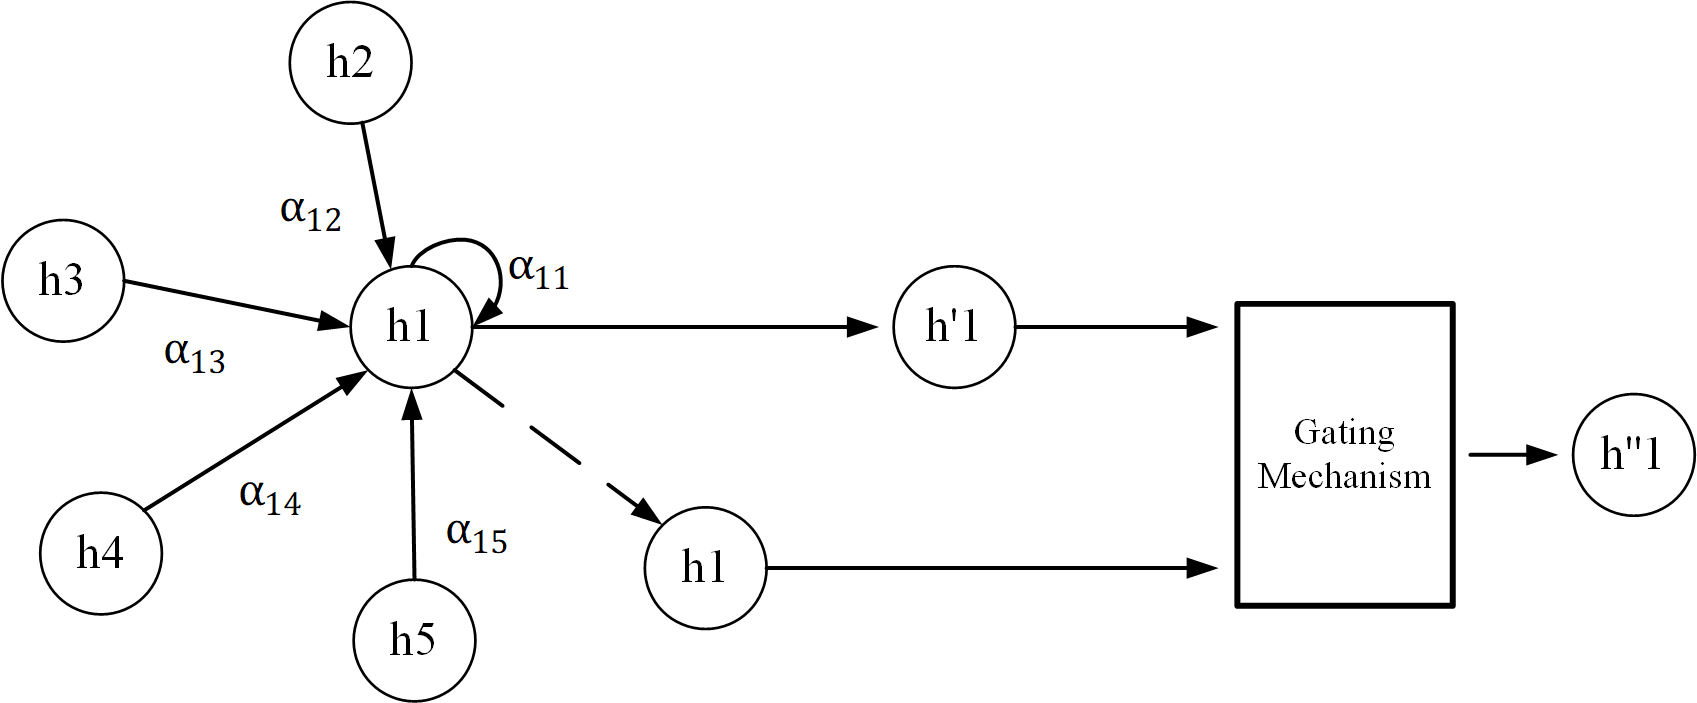
\includegraphics[width=1\textwidth]{pic/attgcn.png}
	\caption{方面级情感分析算法模型}
	\label{attgcn}
\end{figure}
节点向量为$h1$,它的邻居节点向量分别是$h2$、$h3$、$h4$、$h5$。为了选择最当前节点最重要的邻居节点,本章中采用多头注意力机制去计算,获取不同邻居节点对当前节点的权重。首先,
当前节点的向量及其邻居节点向量经过一个线性变化得到注意力机制中的q、k向量,每个向量的计算过程如公式\ref{4attQ}和公式\ref{4attK}所示。其中$W_Q$和$W_K$均是一个维度大小$d\times n$的参数矩阵。
\begin{equation}\label{4attQ}
    q = W_Qh_i, W_Q\in \mathbb{R}^{d\times n}
\end{equation}
\begin{equation}\label{4attK}
    k_i = W_Kh_i, W_K\in \mathbb{R}^{d\times n}
\end{equation}

本章计算方式中查询向量q是指当前节点向量$h1$变换后得到,而对于k向量是当前节点以及当前节点的所有邻居节点的线性变换,因此对于这些节点得到一个
$d*m$的矩阵K,其中$d$为向量维度大小,$m$是指节点个数,如图\ref{attgcn}所示,$m$为5。于是可以得到每个节点对应的注意力分数$\alpha_i$,计算公式如\ref{4attscore}所示。其中$leakyRelu$是一种激活函数。
计算方式如公式\ref{4attleakyRelu}所示,$c$是一个超参数,通常取0.001。
\begin{equation}\label{4attscore}
    \alpha_i = \frac{exp(leakyRelu(\mathbf{q}^\mathsf{T}k))}{\sum_{j}exp(leakyRelu(\mathbf{q}^\mathsf{T}k))}
\end{equation}

\begin{equation}\label{4attleakyRelu}
y_i =
\begin{cases}
x_i & \text{$x_i>=0$} \\
\frac{x_i}{c} & \text{$x_i<0$}
\end{cases}
\end{equation}

再将所有节点的向量输入一个线性变换得到v值,计算方式如公式\ref{4attV}所示,其中$W_K$是一个$d\times n$大小的参数矩阵。$tanh$为激活函数。
因此经过注意力机制更新后得到当前节点新的向量表示为$v'$,如公式\ref{4atth}所示。因为本章使用多头注意力机制,因此有多个注意力计算参与,其中
线性变换参数均有不同,因此最终该节点的向量表示应该为$h'= concat(v'_1,v'_2,...,v'_t)$,其中$t$代表$t$头注意力机制。
\begin{equation}\label{4attV}
    v_i = tanh(W_Vh_i), W_V\in \mathbb{R}^{d\times n}
\end{equation}

\begin{equation}\label{4atth}
    v' = \sum_{j}v_j* \alpha_j
\end{equation}

考虑到多层的GCN网络,每增加一层的计算,当前节点便会获取到更远邻居的信息,而远处节点的信息不一定对当前节点有用,同时还可能导致信息平滑问题,即
当层数深且图较小时,同一连通分量内的节点的表征会趋向于收敛到同一个值\citing{kipf2016semi}。这是由于一方面当前节点容易过多的吸收其他邻居节点的信息而损失了自身节点信息,
另一方面层数加深后,当前节点会获取到更广泛的其他节点信息,这就导致不同节点可能会收到相同的一组邻居节点的信息,使得信息趋于相同。已有部分工作用以解决
这种问题\citing{2018arXiv180603536X,Li_2019_ICCV}。本章采用门控机制,利用GRU中的一个更新门和一个重置门去处理这种问题。首先将GCN网络每一层中
当前节点经过注意力机制更新后的向量$h'$即如图\ref{attgcn}中的向量$h'1$和当前节点处理前的向量$h$即如图\ref{attgcn}中的向量$h1$进行拼接,得到$h_c$,如公式\ref{hconcat}所示。
\begin{equation}\label{hconcat}
    h_c = concat(h',h)
\end{equation}

之后将这个向量分别输入到更新门和重置门,计算过程如公式\ref{ztformul}和公式\ref{rtformul}所示。其中$z_t$和$r_t$分别表示更新门和重置门。$W_{zt}$、$W_{rt}$分别为
更新门和重置门的参数矩阵。$sigmoid$为激活函数,取值为0-1之间,计算如公式\ref{sigmoid}所示。
\begin{equation}\label{ztformul}
    z_t = sigmoid(W_{zt}h_c)
\end{equation}

\begin{equation}\label{rtformul}
    r_t = sigmoid(W_{rt}h_c)
\end{equation}

\begin{equation}\label{sigmoid}
    s = \frac{1}{1+exp(-x)}
\end{equation}

其中更新门用于控制前一层的节点信息被带入到当前层中的程度,更新门的值越大说明前一层的状态信息带入越多,因此得到当前节点的候选集$\tilde{h_t}$,计算如公式\ref{sht}所示。
其中$W_h$为参数矩阵,$concat$为拼接函数。
重置门控制前一层有多少信息被写入到当前的层节点信息候选集上$\tilde{h_t}$,重置门越小,前一状态的信息被写入的越少,因此可以得到最终的节点向量表示$h_t$,如公式\ref{shtt}所示。

\begin{equation}\label{sht}
    \tilde{h_t} = tanh(W_hconcat(z_t*h,h'))
\end{equation}

\begin{equation}\label{shtt}
    h_t = (1-r_t)*h'+r_t*\tilde{h_t}
\end{equation}

$h_t$即为每一层GCN的输出,经过最后一层GCN网络,将会得到一个超节点向量$e_c$和文本中的所有单词向量矩阵$E_w$,其中第i个单词的输出向量为$e_i$。

\subsection{向量融合及分类}
超节点向量$e_c$可以视作是方面词的信息向量,一段文本中对于某个方面词的情感倾向应该取决于文本中的某个词或者多个词,而方面词本身大多数仅仅是一个名词,而没有情感色彩。因此
需要通过方面词的信息从上下文中找出能代表这个方面词情感的词汇。故而本节依然采用一个多头注意力机制进行查找。通过方面词向量关注对这个词具有感情描述的其他的词汇。因此通过
注意力机制可以最终得到表示整个文本情感色彩的向量$e_a$,计算过程如公式\ref{a1},\ref{a2},\ref{a3}所示。其中$W'_q$、$W'_k$、$W'_v$均为用以线性变换的参数矩阵。
\begin{equation}\label{a1}
    a_i = \frac{(W'_qe_c)^\mathrm{T}(W'_ke_i)}{\sqrt{n}}
\end{equation}

\begin{equation}\label{a2}
    \alpha_i = \frac{a_i}{\sum_{j}exp(a_j)}
\end{equation}

\begin{equation}\label{a3}
    e_a = \sum_{j}tanh(W'_vv_j)* \alpha_j
\end{equation}

最终将超节点向量$e_c$和向量$e_a$进行拼接输入到线性变化层以及一个softmax函数得到最终输出向量,其中每一维的数值代表预测归属于某一类别标签的概率,本章算法中选择预测概率
最高的标签作为预测标签,以实现方面级情感分类任务。计算过程如公式\ref{eo},\ref{output}所示。其中$W_o$为输出层的权重矩阵,$b_o$为偏置。
\begin{equation}\label{eo}
    e_o = concat(e_c,e_a)
\end{equation}
\begin{equation}\label{output}
    O = softmax(W_oe_o+b_o)
\end{equation}

该模型利用反向传播(BP)算法进行参数更新,同时使用了Dropout防止模型过拟合。模型迭代N次,直至收敛,最终模型即可在测试集上验证分类效果,实现方面级情感分析任务。

\section{实验设置}
\subsection{数据集描述及数据处理}
本章使用方面级情感分析任务中常用的数据集,包括Twitter数据集,其由Dong等人构建而来\citing{dong-etal-2014-adaptive},以及另外三种数据集,LAP 14,Rest 14,Rest 15。
LAP 14和Rest 14来自于SemEval 2014 task 4\citing{pontiki-etal-2014-semeval},Rest 15来自于SemEval 2015 task 12\citing{pontiki-etal-2015-semeval},这四种数据集
均为英文数据集。本章分别在这四种数据集上进行验证模型及与其他模型进行对比。

\textbf{Twitter}数据集来自于Twitter上的一些关于名人、产品和公司等评论。总共有6940个文本,其中训练集包含6248段文本以及692个测试集。
该数据集共有三种类别,分别是正向情感,负面情感以及无情感倾向。以文本“i love my kindle , i really do .”为例,在这个数据集中,对应的方面词为“kindle”,
对应的标签为“1”,即正面情感。该数据集即需要根据给出的方面词,判断这个方面词在这段文本中所包含的情感色彩。

\textbf{LAP 14}数据集主要是关于电脑方面的一些评价。总共有2966个文本,其中测试集638个,2328个训练集。与twitter数据集一致,依然是正向、负面以及
无情感三种类别。以句子“it is the perfect size and speed for me”为例,其中“perfect”为方面词,其对应的标签为“1”,即正面情感,可以从单词“perfect”得出
这个结论。

\textbf{Rest 14和Rest 15}两种数据集来自于不同的年份的关于餐厅的评论。Rest 14包含4728个样本,其中共计3608个训练集以及1120个测试集。
Rest 15包含1746个样本,其中包括1204个训练集以及542个测试集,两者均与上类似为3类标签。数据集中的样本如句子“i recommend this place to everyone”为例,这个句子中给定的方面词为“place”,
从整个句子可以分析出,对于这个方面词给予的是正面评价,这从给定的标签为“1”得到验证。

数据集中详细统计如表\ref{summaryAspect}所示。
\begin{table*}[htb]
	\centering
	\caption{数据集数据统计}
	\setlength{\tabcolsep}{4mm}{
		\begin{tabular}{c|c|c|c|c}
			\hline 
			{数据集} & {划分} & {正向}& {负向} & {无倾向}   \\
			\hline 
			\multirow{2}*{$ \text{Twitter} $}
			& 训练集 & $  1561$ & $  1560 $& $ 3127 $    \\ 
			~ & 测试集 & $   173$ & $  173 $& $ 346 $    \\ \hline
			\multirow{2}*{$ \text{LAP14} $}
			& 训练集 & $  994$ & $   870 $& $ 464 $    \\ 
			~ & 测试集 & $   341$ & $   128 $& $ 169 $    \\ \hline
			\multirow{2}*{$ \text{Rest 14} $}
			& 训练集 & $  2164$ & $  807 $& $ 637 $    \\ 
			~ & 测试集 & $   728$ & $  196 $& $ 196 $    \\ \hline
			\multirow{2}*{$ \text{Rest 15} $}
			& 训练集 & $  912$ & $  256 $& $ 36 $    \\ 
			~ & 测试集 & $   326$ & $   34 $& $ 182 $    \\ \hline
		\end{tabular}%
		\label{summaryAspect}%
	}
\end{table*}

本章使用的文本预处理方式与第三章中采用用的方式一致。如果使用Glove作为单词初始化向量时,会对数据集中的所有的单词进行一个唯一编号,同时将文本按照“空格”分词后,按照单词索引找出对应的单词向量。
文本就由一组单词向量组成。同时超节点的向量采用零向量进行初始化。如果采用BERT的预训练模型,则输入到GCN中的单词向量为BERT模型最后一层的输出,并且超节点向量依然采用零向量进行初始化。

\subsection{对比方法介绍}
本章提出的方法是针对于方面级情感分析任务。因此对比的方法均是近些年常用于比较的模型,且同时比较了采用例如word2vec或glove作为词向量初始化的模型以及采用基于BERT预训练模型的方法。主要比较模型如下:

\textbf{SVM:}Kiritchenko等人\citing{Kiritchenko-svm}提出的一种基于支持向量机的方面级情感分析算法。

\textbf{LSTM:}Tang等人\citing{tang2015effective}提出的一种基于LSTM模型的算法,该算法使用了LSTM模型的最后一层的隐藏状态向量作为分类向量实现情感极性判断。

\textbf{MemNet:}Tang等人\citing{tang-etal-2016-aspect}提出采用一个深层注意力机制捕捉方面词与文本单词之间的关系。相比于基于特征工程的SVM和基于序列单元的LSTM,它们提出的模型
在推断一个方面词的情感极性时,更能明确地抓住每个重要的上下文单词。

\textbf{AOA:}Huang等人提出了一个AOA(Attention-over-Attention)模型,该模型采用Bi-LSTM模型以及注意力机制进行捕捉到方面目标词与文本内容之间的关系信息,从而推断那些词对于方面词情感分析有帮助。

\textbf{IAN:}Ma等人\citing{Ma2017Interactive}提出的基于注意力机制的方法将方面词以及文本上下文内容共同建模,将两者信息交互起来学习,实现多层次语义分析。

\textbf{Tnet-LF:}Li等人\citing{li2018transformation}提出了一个上下文持久化持变换(Context-Preserving Transformation,CPT)的概念,保留和加强部分上下文信息。
每个CPT层包含一个Bi-LSTM模型,该模型用以处理方面级的目标词,获取目标词的向量表示。然后将这个向量表示与输入的单词向量进行拼接输入到一个全连接层,最终生成一个新的向量表示,
该向量体现了每个单词与目标词之间的关系信息。随后再对CPT输出的这组向量表示采用CNN模型卷积处理,捕捉关键信息,生成表示文本的向量。

\textbf{ASGCN-DT:}Zhang等人\citing{zhang2019aspect}提出采用解析树的方式构建文本图,以利用句法信息和单词依存关系,并使用图卷积神经网络(GCN)用以学习方面目标单词与文本内容单词之间的关系。

\textbf{TG-BERT:}Gao等人\citing{Gao2019Target}提出的一种基于BERT的模型。该模型将BERT模型中输出的方面词向量采用最大池化的方式挑选最重要的特征生成一个向量,然后结合BERT模型中的
cls向量输入到一个全连接层实现分类任务。

\textbf{DGEDT(BiGCN):} Tang等人\citing{tang2020dependency}提出的一种基于双向GCN的模型。该模型采用语法解析树的方式构建图,解析树生成的单词之间联系有着前后关系,因此考虑到这种关系,
采用了一种双向GCN提取信息。通过GCN学习单词向量表示以及方面词向量表示,再结合一个注意力机制提出关键信息,实现情感分类任务。

\textbf{DGEDT-BERT:}相比于DGEDT(BiGCN)模型,该模型结合了一个transformer结构,即一方面采用transformer结构学习单词向量表示,另一方面再采用一个双向GCN模型学习单词向量表示,接着采用
他们提出的一个BiAffine模块,将两种方式学到的单词向量融合起来,得到更加具有丰富表示的单词向量。同时,该模型还结合了BERT预训练模型,将BERT模型的单词输出作为transformer结构和GCN结构的
输入,进一步提升模型分类性能。

\textbf{GAGCN及GAGCN-BERT:}GAGCN即为本章提出的算法模型,GAGCN-BERT代表使用了BERT模型的单词输出作为GAGCN模型中的单词输入,其他结构不变。

各类模型详细统计如表\ref{summaryMethod}所示。
\begin{table*}[htb]
	\centering
	\caption{算法模型统计}
	\setlength{\tabcolsep}{4mm}{
		\begin{tabular}{c|c|c|c|c}
			\hline 
			{模型} & {使用LSTM} & {使用GCN}& {使用注意力机制} & {使用BERT}   \\
			\hline 
			$ \text{SVM} $ &  $\times$  &  $\times$ &  $\times$  &  $\times$   \\ \hline
			$ \text{LSTM} $&  $\checkmark$ &  $\times$  &  $\times$  &  $\times$   \\\hline
          	$ \text{MemNet} $& $\times$  &  $\times$  &  $\checkmark$  &  $\times$   \\\hline 
			$ \text{AOA} $& $\checkmark$ &  $\times$  &  $\checkmark$  &  $\times$    \\\hline 
			$ \text{IAN} $ &  $\checkmark$  &  $\times$ &  $\checkmark$  &  $\times$   \\ \hline
			$ \text{Tnet-LF} $&  $\checkmark$ &  $\times$  & $\checkmark$  &  $\times$ \\\hline
			$ \text{ASGCN-DT} $& $\checkmark$ &  $\checkmark$ &  $\checkmark$  &  $\times$   \\\hline 
			$ \text{TG-BERT} $& $\times$  &  $\times$  &  $\times$   &  $\checkmark$   \\\hline 
			$ \text{DGEDT(BiGCN)} $& $\checkmark$ &  $\checkmark$ & $\checkmark$ &  $\times$   \\ \hline 
			$ \text{DGEDT-BERT} $& $\times$ &  $\checkmark$ &  $\checkmark$  &  $\checkmark$   \\\hline 
			$ \text{GAGCN} $& $\times$ &  $\checkmark$ &  $\checkmark$  &  $\times$   \\\hline 
			$ \text{GAGCN-BERT} $& $\times$ &  $\checkmark$ &  $\checkmark$  &  $\checkmark$   \\\hline 
		\end{tabular}%
		\label{summaryMethod}%
	}
\end{table*}

\subsection{模型参数设置及评价指标}
对于本章提出的算法GAGCN未使用BERT模型输出的词向量,因此采用了300维的Glove词向量作为单词的初始化。对于使用了BERT模型的GAGCN-BERT,将BERT模型的最后一层词向量作为GAGCN词向量的
输入。BERT模型本章与GAGCN结合,训练过程中进行微调,BERT参数的学习率为0.00002。而GAGCN模型的参数学习率为0.0001,且训练过程中Dropout为0.5。文本建模图过程中的滑动窗口大小定为5,滑动窗口中
每组单词权重设置为0.2。GCN层数采用2层。其他模型均使用各自论文中的实验结果。

为了测试模型之间的性能,所有数据集均按照标准的划分方式划分为训练集和测试集,模型在训练集上进行训练,在测试集上进行验证。

为验证模型参数的影响,实验中设置了不同大小的网络神经元个数进行方法的对比实验,分别设置了64,128,256,512,768个神经元个数。此外,本章算法中提出使用了一个特别的训练技巧,即数据扩充。因为训练样本有限,数据扩充能一定程度上使模型泛化能力更强,进而提升分类性能。
方面词本身并不包含情感色彩,而影响对方面词情感极性判断的决定性因素是文本中的其他词汇。因此方面词所处在的文本位置决定了这个方面词的情感。基于这种思想,该数据扩充方式的实现为,将一段文本
中的方面词替换成另外一个文本中的方面词,保证替换后所处的文本位置不变。为验证这种思想的正确性,实验对比了采用数据扩充以及未使用数据扩充的模型。

对于实验效果的评估,与第三章一致,使用准确率(accuracy)和macro-F1分数来验证模型的分类性能。

\section{实验结果及分析}
\subsection{模型分类性能分析}
本小结对于未使用BERT模型的GAGCN采用Glove词向量作为单词向量初始化,其他对比方法使用论文中的实验数据。

\begin{table*}[htb]
    \centering
    \caption{各模型分类性能比较}
    \renewcommand\arraystretch{1}
    \renewcommand\tabcolsep{2mm}
    \label{tab:gagcn-result}
    \arrayrulecolor{black}
    \begin{tabular}{lcccccccc}
    \hline
    \multirow{2}{*}{\textbf{Models}} & \multicolumn{2}{c}{\textbf{TWITTER}} & \multicolumn{2}{c}{\textbf{LAP14}} & \multicolumn{2}{c}{\textbf{REST14}} & \multicolumn{2}{c}{\textbf{REST15}}  \\
    \cline{2-9}
                            & ACC   & F1-score       & ACC   & F1-score        & ACC   & F1-score       & ACC   & F1-score          \\
    \hline
    SVM                 & 63.4 & 63.3         & 70.49 & -          & 80.16 & -         & -     & -                 \\
    LSTM                 & 69.56 & 67.7         & 69.28 & 63.09 & 78.13 & 67.47         & 77.37 & 55.17           \\
    AOA                     & 72.3 & 70.2         & 72.62 & 67.52          & 79.97 & 70.42         & 78.17 & 57.02            \\
    IAN                    & 72.5 & 70.81         & 72.05 & 67.38          & 79.26 & 70.09         & 78.54 & 52.65            \\
    Tnet-LF                 &72.98  & 71.43         & 74.61 & 70.14          & 80.42 & 71.03         & 78.47 & 59.47            \\
	ASGCN-DT                   & 72.15 & 70.4         & 75.55 & 71.05          & 80.77 & 72.02          & 79.89 & 61.89            \\
	MemNet                   & 71.48 & 69.9         & 70.64 & 65.17          & 79.61 & 69.64          & 77.31 & 58.28            \\
	DGEDT(BiGCN)                     & 72.8 & 71         & 76.2 & 71.8           & 81.8 & 72.5        & 80.4  & 62.9            \\
	GAGCN                     & 73.22 & 71.66         & 76.12 & 71.46           & 81.61 & 73.29         & 80.63  & 61.45           \\
    \hline
	TG-BERT                   & 76.7 & 74.3         & 78.9 & 74.4          & 85.1 & 78.4         & - & -            \\
	DGEDT-BERT                   & \textbf{77.9} & \textbf{75.4}         & \textbf{79.8} & 75.6          & \textbf{86.3} & 80         & 84 & 71            \\
	GAGCN-BERT                   & 76.45 & 74.89         & 79.6 & \textbf{75.86}         & 86.25 & \textbf{80.14}         & \textbf{85.23} & \textbf{72.25} \\
    \hline
    \end{tabular}
    \arrayrulecolor{black}
	\end{table*}
	
如表\ref{tab:gagcn-result}所示,展示了不同模型之间的准确率(ACC)和 F1 分数(F1-score)。此表中GAGCN和GAGCN-BERT方法隐藏层中采用的神经元数为768,注意力机制头数为8。

如表\ref{tab:gagcn-result}所示,对于采用了BERT预训练模型的方法明显在准确率以及F1分数上高于其他未使用BERT模型的方法。说明BERT预训练模型的使用能极大地提升方法的性能。
这是由于BERT模型采用了大量的数据进行预训练,配合下游任务可以实现更快的收敛速度,从而能够有效地提高模型性能。同时BERT模型对于每个单词对应都会生成一个词向量,即使一个文本中
同一个单词出现在不同的位置,那么这个单词就会有多个词向量,体现了单词在文本上下文中位置的不同而产生的不同含义,而Glove每个单词仅有唯一的一个词向量,忽略了一个单词可能在不同语境下
具有不同的含义。例如“apple”一词,可能指一种水果,也可能指的是公司名。含义取决于上下文,而BERT模型就考虑了上下文关系。此外,从表中可以看出,对于使用GCN模型的方法,如ASGCN-DT、DGEDT(BiGCN)
和GAGCN实验效果均表现不错,
这是由于这几种方法中通过构建文本图的过程就建立了一种上下文关系,无论是使用滑动窗口构图,或是依赖解析树构图,均展现了单词之间的上下文关系。再通过GCN网络节点之间的信息传递,单词之间的
信息进行流动,将这种上下文关系融入至单词词向量中,学得更加丰富的单词向量表示。有利于提升模型性能。

对于未采用BERT模型,而使用了GCN的模型来看,本章提出的GAGCN展现了较为优异的性能。相比于ASGCN-DT,基本在所有数据集上的准确率和F1分数都更为优秀,尤其是在Twitter数据集上,准确率提升了1.07\%。
但是在REST15数据集上,F1分数相对较低。对比DGEDT(BiGCN)模型,GAGCN互有优势,在Twitter和REST15数据集的准确率上,GAGCN表现更好,但是其他数据集略微不足,不过差距都不大。相比于其他模型,这三种使用
GCN的方法无论是准确率或是F1分数,均有明显的优势。而DGEDT(BiGCN)和ASGCN-DT均使用了LSTM模型提取单词的隐藏向量表示,LSTM是序列模型,在计算中无法实现并行运算,这将影响运算性能,而GAGCN未使用LSTM架构,
故在不影响过多分类性能的情况下展现了更好的计算效率。

对于TG-BERT、DGEDT-BERT和GAGCN-BERT这三种使用BERT预训练模型的方法来说,DGEDT-BERT和GAGCN-BERT分类性能更具优势,基本都高于TG-BERT,尤其是在REST14数据集上,这两个方法的准确率高于TG-BERT接近1.2\%。
由于TG-BERT只是简单地将BERT模型输出的方面词向量进行了池化以及与cls向量拼接进行分类,一定程度上忽略了方面词与文本中的其他词汇的关系。而DGEDT-BERT和GAGCN-BERT不仅通过GCN网络学习到了更加
丰富的词向量表示,还采用了注意力机制,挖掘对方面词具有分类帮助的词汇。DGEDT-BERT相比于GAGCN-BERT多了一个transformer结构,这将明显增加计算资源消耗,当计算资源较为贫乏时,GAGCN更具优势。此外
DGEDT-BERT采用语法依赖解析树的方式进行文本构图,构图的效果取决于使用的语法解析方法的好坏,而GAGCN-BERT采用的是滑动窗口方式构图。GAGCN也采用过语法解析树的方式生成图,但实际效果远不如
滑动窗口的方式,因此对于这两种构图的方式呈现的效果可能取决于具体的模型架构。

\subsection{GAGCN中使用的GCN与普通GCN对比}
GAGCN方法中使用的GCN包含了注意力机制以及一个门控机制,为对比这两个机制对模型性能的提升,本节实验与普通的未使用注意力机制和门控机制的GCN进行对比。这两个对比方法,均未
使用BERT预训练模型,仅在GCN模型上有差异,即是否使用了注意力机制和门控机制,算法的其他部分一致——即采用了相同的文本处理方法、构图方式以及最终的向量融合方式和分类方法。
% \begin{figure*}[htb]
%     \begin{minipage}[t]{0.5\linewidth}
%     \centering
%     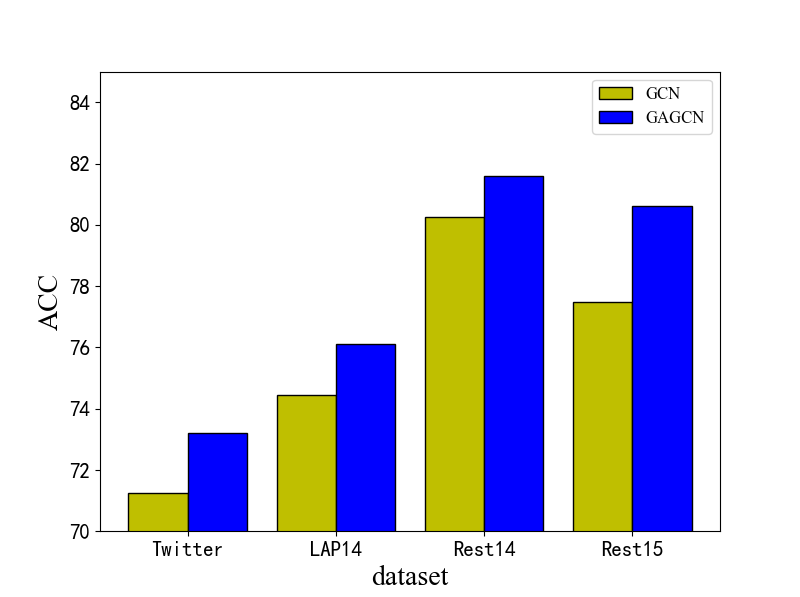
\includegraphics[width=1\textwidth]{pic/gcn-gagcnAcc.png}
%     \caption{分类准确率(ACC)}
%     \label{gcn_gagcn_acc}
%     \end{minipage}
%     \quad
%     \begin{minipage}[t]{0.5\linewidth}
%     \centering
%     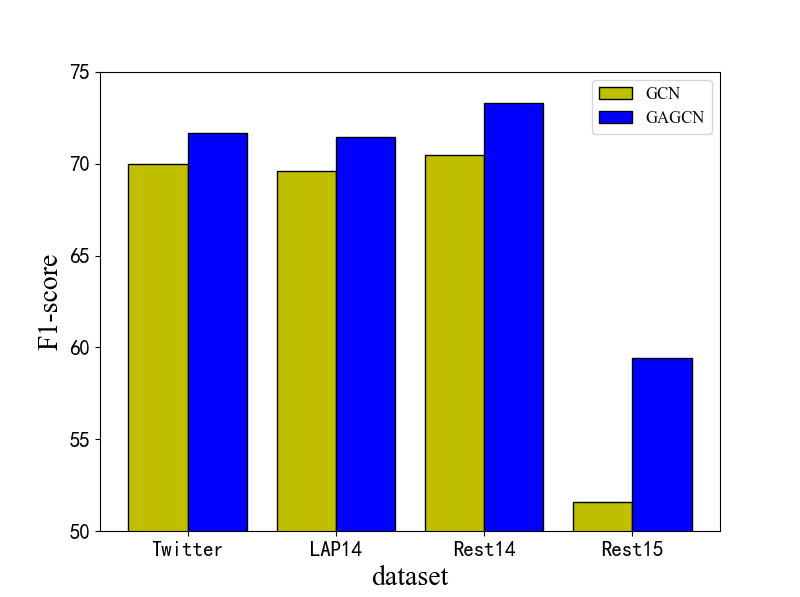
\includegraphics[width=1\textwidth]{pic/gcn-gagcnF1.png}
%     \caption{分类F1分数(F1-score)}
%     \label{gcn_gagcn_f1}
%     \end{minipage}
% \end{figure*}

\begin{figure}[htb]
    \setlength{\belowcaptionskip}{0pt}
    \centering
    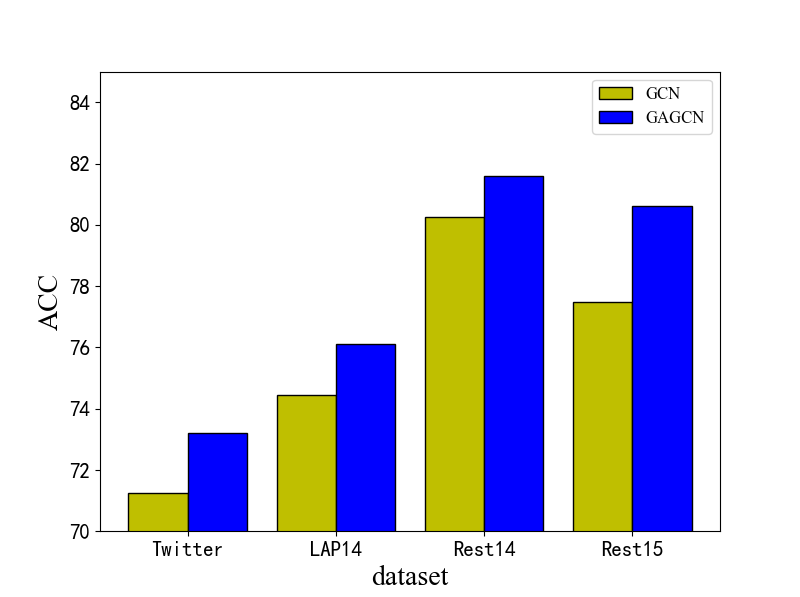
\includegraphics[width=0.8\textwidth]{pic/gcn-gagcnAcc.png}
    \caption{分类准确率(ACC)}
    \label{gcn_gagcn_acc}
\end{figure}

\begin{figure}[htb]
    \setlength{\belowcaptionskip}{0pt}
    \centering
    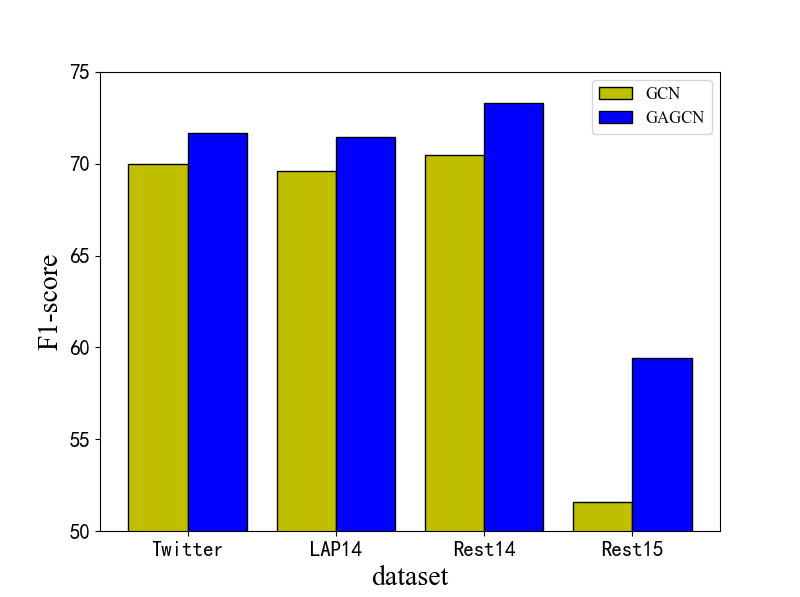
\includegraphics[width=0.8\textwidth]{pic/gcn-gagcnF1.png}
    \caption{分类F1分数(F1-score)}
    \label{gcn_gagcn_f1}
\end{figure}

如图\ref{gcn_gagcn_acc}所示,展示了GAGCN与普通GCN方法的准确率。从图可以看出,在所有的数据集的结果中,GAGCN都明显高于普通的GCN,尤其是在Rest15数据集上高出了3.14个百分点。
说明GAGCN的注意力机制能够辅助模型找到对当前节点贡献度较高的邻居节点,并更多的获取来自这个邻居节点的信息,同时门控机制控制了当前层与上一层节点信息的选取,自适应选择机制可以
帮助模型选择每一层网络中重要的节点信息。F1分数的结果如图\ref{gcn_gagcn_f1},与准确率的结果一致,GAGCN显著高于普通的GCN,
且在Rest15数据集上高出了7.87\%。因此这两个图结果都能证明GAGCN注意力机制和门控机制的有效性。在图节点信息的传播过程中,通过注意力机制挖掘邻居节点之间的关联程度,辅助节点获取到更关键的信息,有助于提升模型性能。

\subsection{数据增扩效果验证}
本节对GAGCN-BERT中提出的数据增扩方法进行了验证。两种形式的参数设置一致,仅有的差异即是在训练过程中是否使用了数据增扩。数据增扩的实现以LAP数据集中的句子“it's color is even cool”为例,这里的
方面词为“color”,在训练的过程中,这句话的方面词有50\%的几率被替换成另一个句子中的方面词,比如“service”,但标签依然维持不变。训练集中的所有句子均有50\%被替换成另一个方面词,而测试集不做替换。
% \begin{figure*}[htb]
%     \begin{minipage}[t]{0.5\linewidth}
%     \centering
%     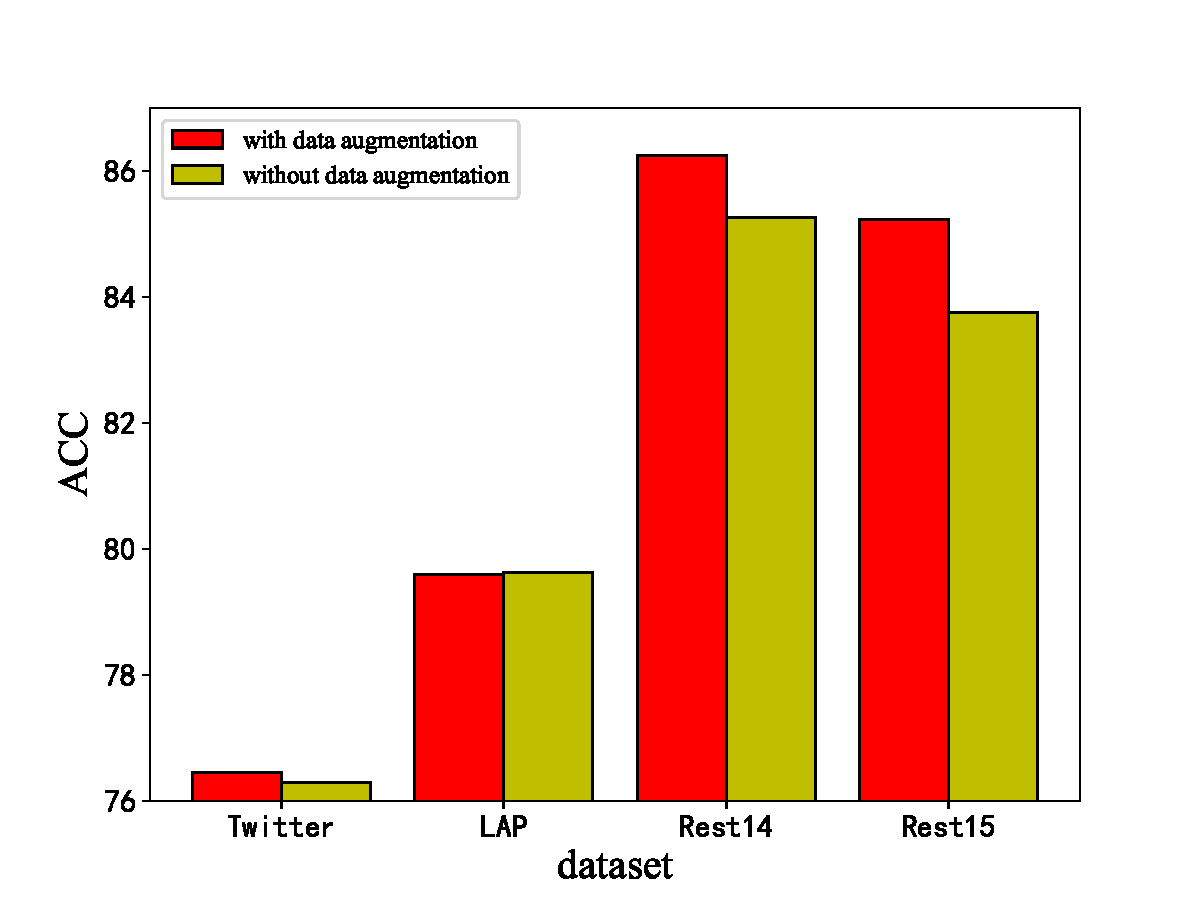
\includegraphics[width=1\textwidth]{pic/DAACC.pdf}
%     \caption{分类准确率(ACC)}
%     \label{DAACC}
%     \end{minipage}
%     \quad
%     \begin{minipage}[t]{0.5\linewidth}
%     \centering
%     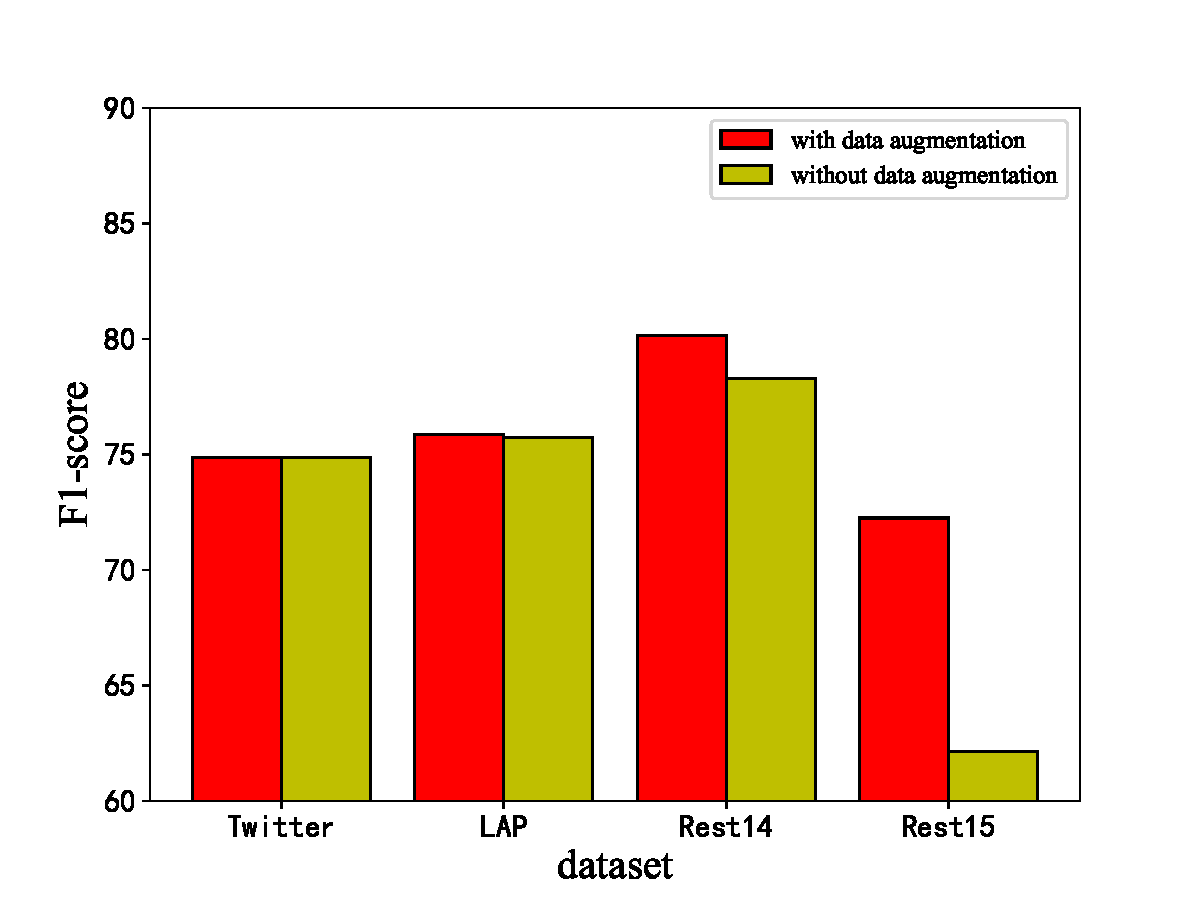
\includegraphics[width=1\textwidth]{pic/DAF1.pdf}
%     \caption{分类F1分数(F1-score)}
%     \label{DAF1}
%     \end{minipage}
% \end{figure*}

\begin{figure}[htb]
    \setlength{\belowcaptionskip}{0pt}
    \centering
    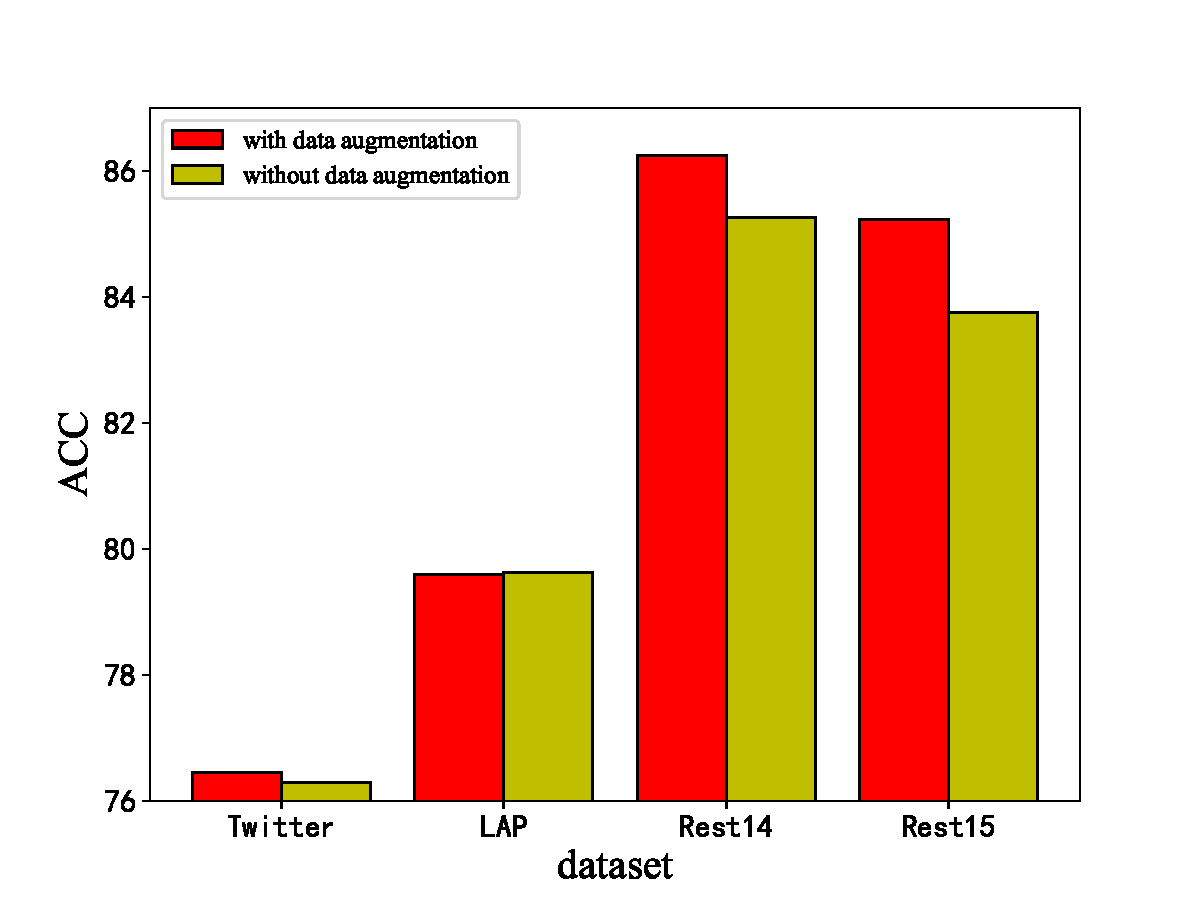
\includegraphics[width=0.6\textwidth]{pic/DAACC.pdf}
    \caption{分类准确率(ACC)}
    \label{DAACC}
\end{figure}

\begin{figure}[htb]
    \setlength{\belowcaptionskip}{0pt}
    \centering
    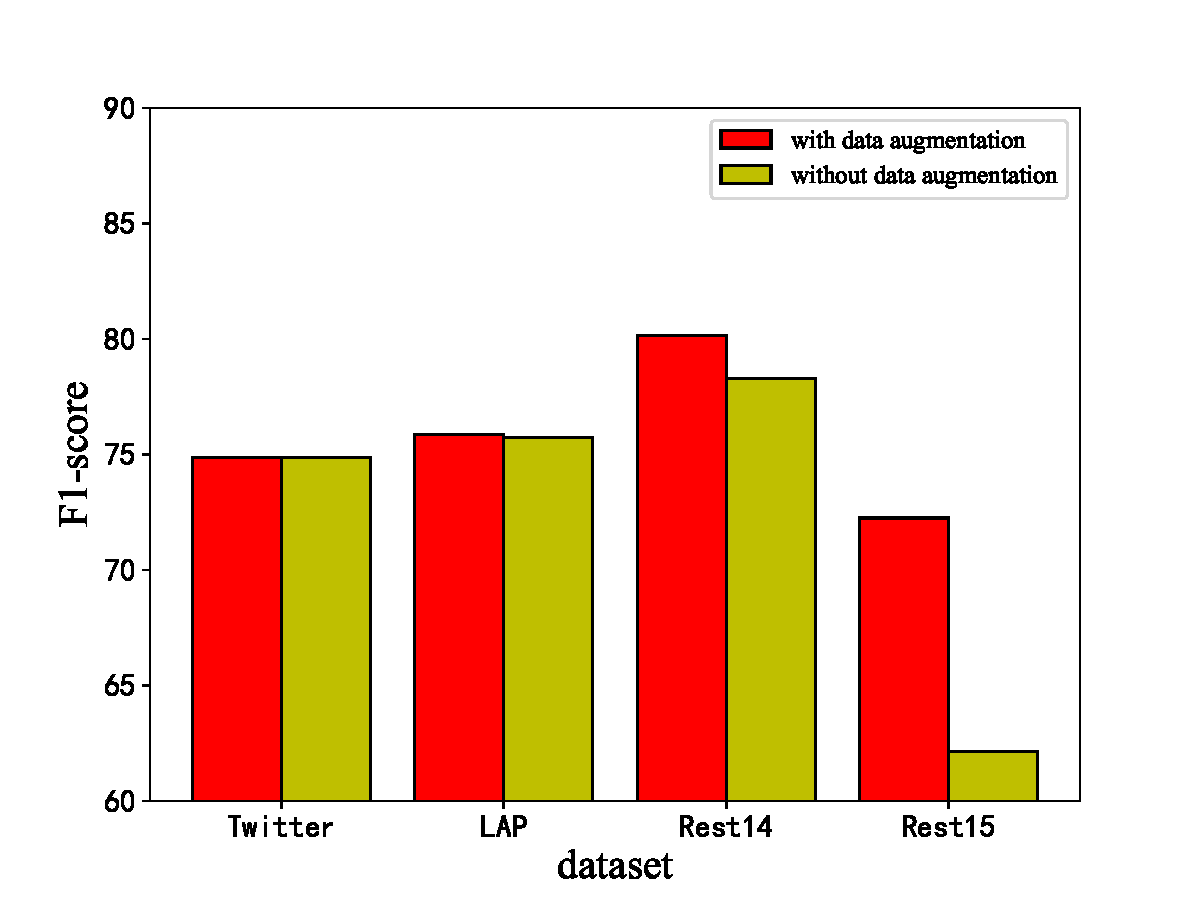
\includegraphics[width=0.6\textwidth]{pic/DAF1.pdf}
    \caption{分类F1分数(F1-score)}
    \label{DAF1}
\end{figure}

如图\ref{DAACC}所示,展示了两种训练方式的分类准确率,从图中可以看出,使用了数据增扩的模型在这四种数据集上基本都高于未使用数据增扩的方法,尤其是在Rest15数据集上,提升了1.47\%。
这可能是由于Rest15数据集相比于其他数据集训练样本更少,模型训练样本不足,容易产生过拟合,故采用数据增扩的方式补充一定量的训练样本,有利于提升模型的泛化能力,提升分类性能。

如图\ref{DAF1}所示,
展示了F1-score的对比差异,与准确率结果类似,使用了数据增扩的方法分类性能优于未使用数据增扩的模型,并且在Rest15数据集上提升了10.1个百分点。差距十分明显。从准确率和F1分数的
结果来看,本章提出的数据增扩方式对模型性能有一定提升,尤其是在仅有少量训练样本的数据集下表现突出。因为这种数据增扩的方式通过替换方面词,让模型学习过程中不过多依赖方面词本身的含义,而去
捕捉语法信息,即方面词所处的上下文位置才是决定情感极性的关键。因此从某种角度上来看这种数据增扩方式一方面增加了训练样本,另一方面引入了人为定义的规则,即让模型不要过多关注于方面词的自身
语义,而去关注于单词间的关系以及语法信息。

\subsection{实验参数比较}
本节比较了不同参数设置条件下模型的分类性能。如图\ref{paraunitacc}所示,比较了设置不同大小神经元个数的GAGCN-BERT模型。由于BERT模型采用的是预训练模型,故未更改BERT中每层网络的神经元个数,而是修改
GAGCN-BERT中GCN每层网络中的神经元个数。

\begin{figure}[htb]
    \setlength{\belowcaptionskip}{0pt}
    \centering
    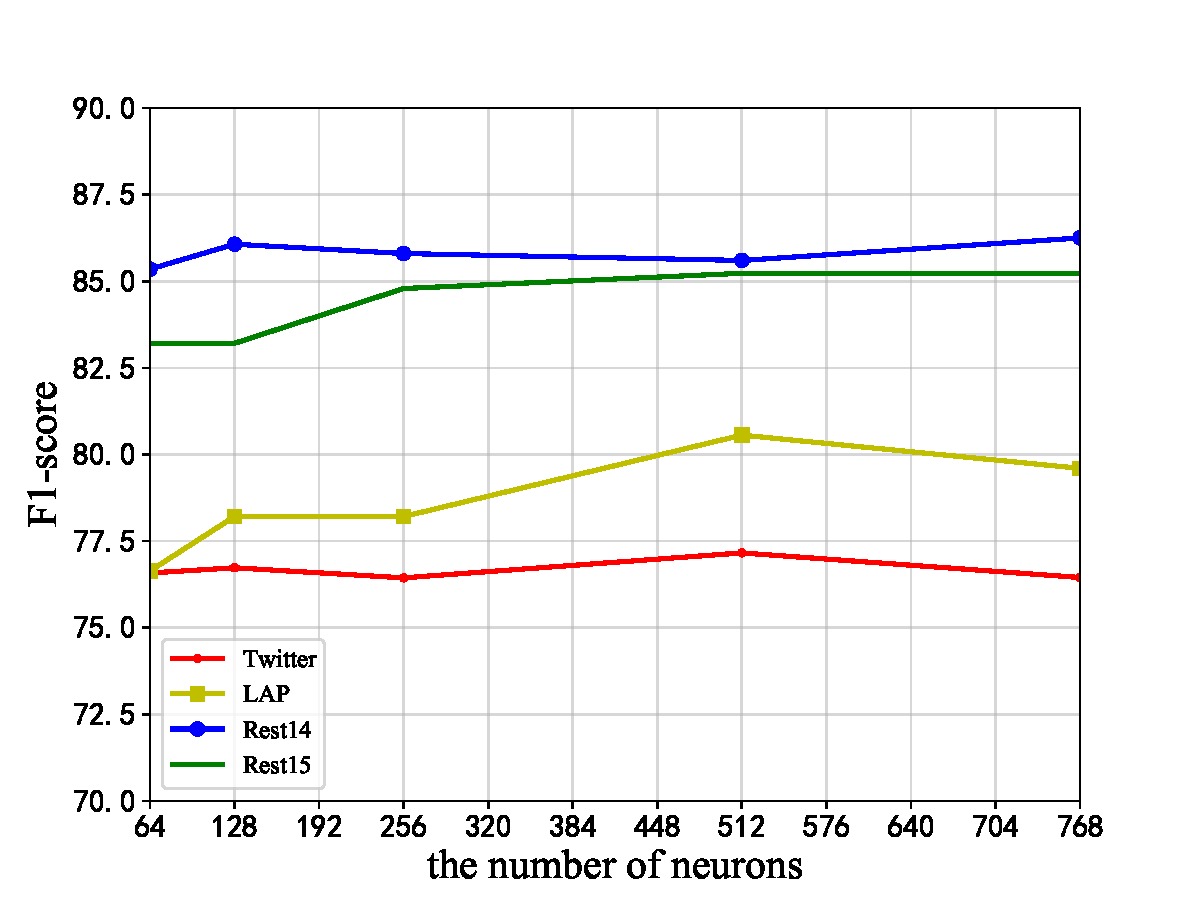
\includegraphics[width=0.6\textwidth]{pic/unitACC.pdf}
    \caption{不同神经元个数比较}
    \label{paraunitacc}
\end{figure}

\begin{figure}[htb]
    \setlength{\belowcaptionskip}{0pt}
    \centering
    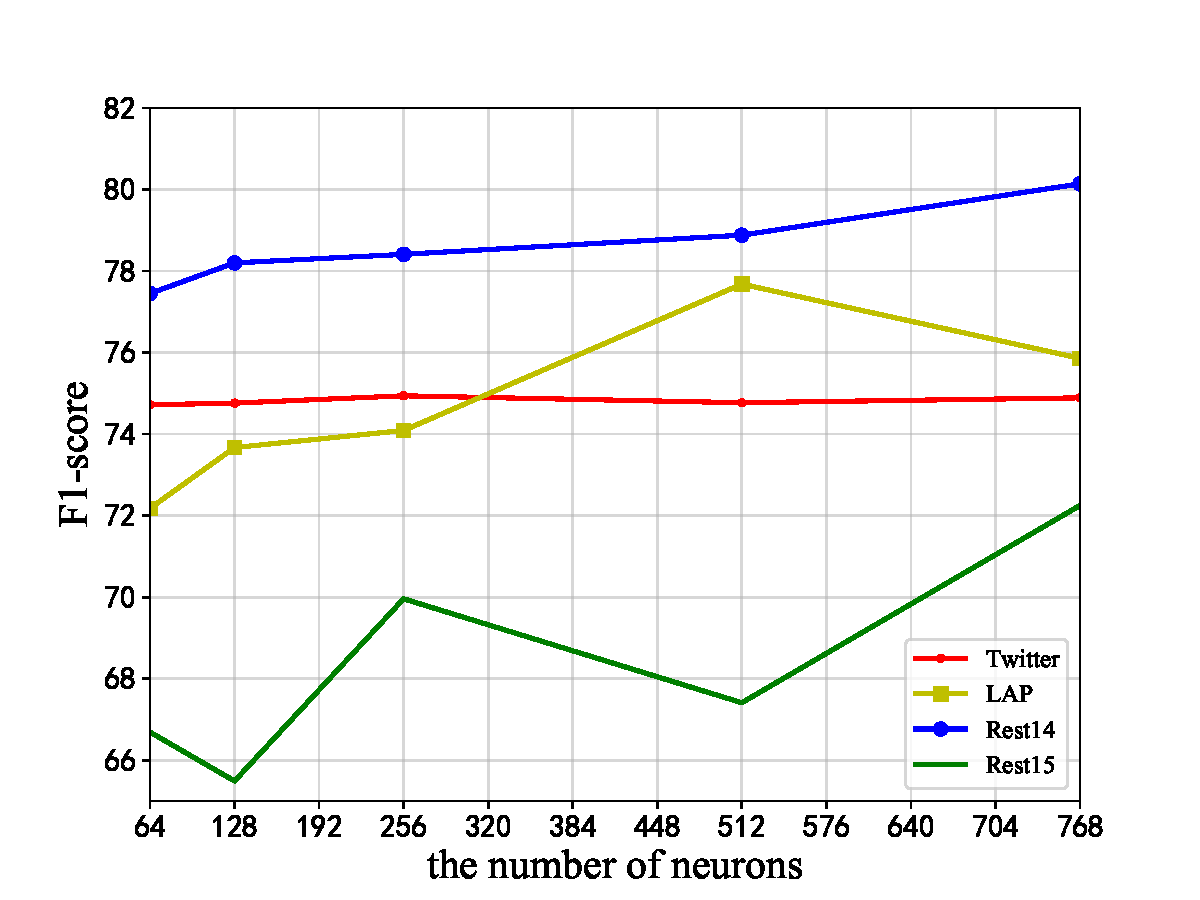
\includegraphics[width=0.6\textwidth]{pic/unitF1.pdf}
    \caption{不同神经元个数比较}
    \label{paraunitf1}
\end{figure}

从图\ref{paraunitacc}中结果来看,该模型的分类准确率对神经元个数不是特别敏感,整体的趋势是随着神经元个数的增加而增加。当神经元个数低于64时分类性能则表现最差,如在LAP数据集上
相比效果最好的模型相差3.92个百分点。这是由于神经元个数非常低时,则所能容纳的信息量将会大幅压缩,从而导致产生的向量信息量较少,无法展现文本数据集
内容信息,故低神经元个数情况下分类性能较差。整体来看,模型在512和768个神经元时表现相对最好。模型F1分数结果如图\ref{paraunitf1}所示。与准确率的趋势一致,整体情况是随着神经元个数的
增加,模型性能也能得到提升。在64个神经元个数时效果最差。

\section{本章小结}
本章介绍了方面级情感分析算法,主要是基于图卷积神经网络以及对第三章算法的延续。建立一个超节点连接方面词中的所有单词,通过GCN网络中节点的信息传递,将方面词中的各个单词进行交互,同时随着
网络层数的加深,也能将超节点的信息传递给文本其他单词,建立超节点与文本上下文中单词之间的联系。注意力机制与门控机制的应用保证节点之间信息的流动具有选择性,即当前节点着重关注于重要的邻居节点,
并从这类节点中获取更多的信息。从结果来看,本章提出的方法在准确率和F1分数上均取得了不错的效果,相比于大多数对比方法均有提升,虽然在部分数据集上不如DGEDT(BiGCN),但是差距细微,且相比之下本章
提出的方法具有更高的计算效率。此外融入了BERT模型进一步提升模型性能,展现了不俗的分类性能。本章还提出了一种数据增扩方式,相比未使用该方法的模型,分类性能有一定的提升。